\chapter{The Standard Model of Physics}\label{chap:SM}

\section{The Theory As It Stands}

The purpose of the LHC and other similar colliders is to study physics at the most fundamental level of existence. We are interested in probing and measuring the smallest building blocks of nature, and in discovering how they go together. The most complete picture which we have to date is shown in Figure~\ref{fig:standard_model}.

\begin{figure*}[htbp]
    \centering
    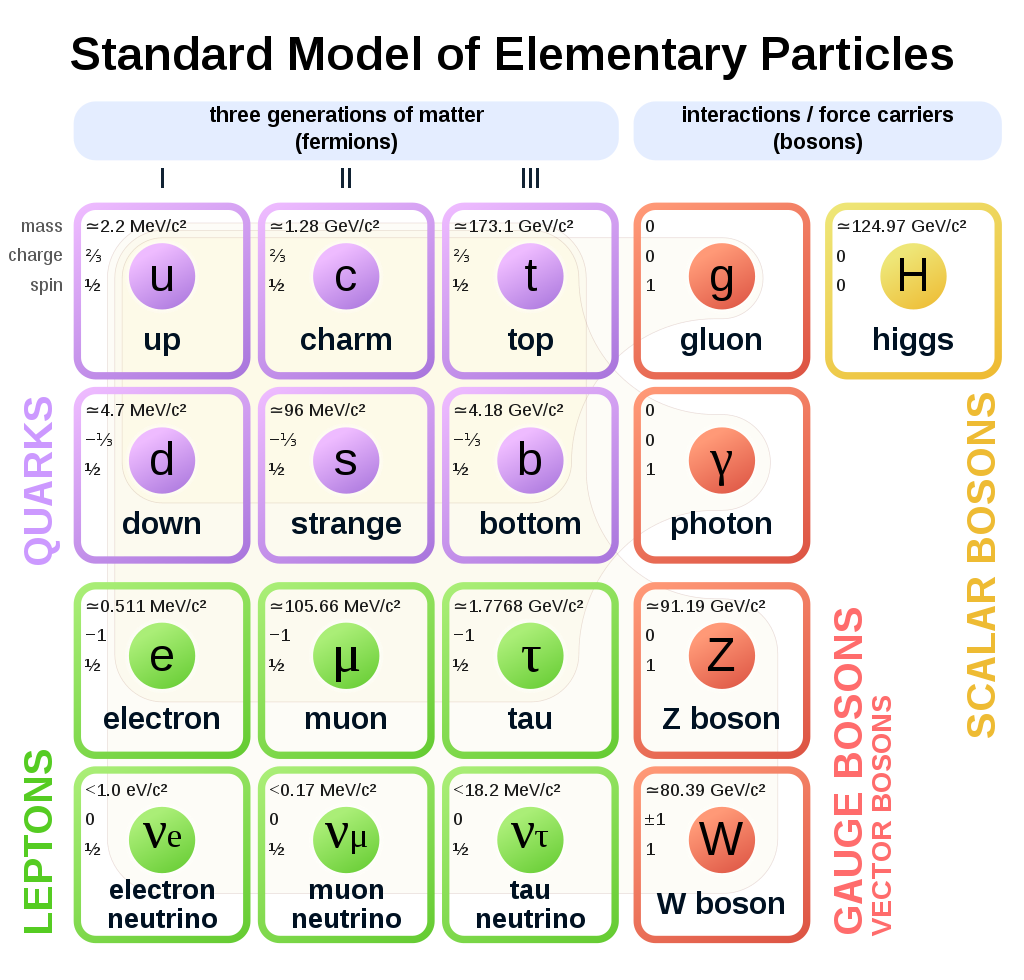
\includegraphics[width=0.7\textwidth]{Images/Background/standard_model.png}
    \caption{The Standard Model.}
    \label{fig:standard_model}
\end{figure*}

In this model, known as the Standard Model, we describe the universe as a composition of particles and the forces between them~\cite{Griffiths}. The leptons, shown in green, include the well-known electron, as well as its nearly-invisible partner, the electron neutrino. Quarks, shown in purple, include the building blocks of protons and neutrons, the up and down quarks. Furthermore, there are the heavier generations of the well-known leptons and quarks, which are just like the electron, electron neutrino, up quark, and down quark, only with more mass. We also have the force carriers (or gauge bosons) in orange - photons for the electromagnetic force, gluons for the strong force, and W and Z bosons for the weak force. Finally, completing the picture is the recently-discovered Higgs boson, an excitation of the Higgs field which gives mass to the other fundamental particles. There are also the antimatter counterparts to these particles, which have opposite charge, though the neutral force carriers are their own antiparticles. The neutrinos may be their own antiparticles too, but whether they are or not is currently the subject of research.

These particles and force carriers, along with the ways in which they are allowed to interact, or "couple" with each other, determine the motion and interaction of all things that we know about in our everyday existence. However, this model is still far from complete, as it does not describe gravity, and is also unable to explain many types of observed astronomical phenomena. Furthermore, there are problems with fine-tuned variables which exist in the model. All of these problems will be described in the next section.

For now though, let's turn our attention to the force carrier particles. These particles are \textbf{describe mixing through electroweak spontaneous symmetry breaking}. This distinction will be important later when we describe supersymmetric extensions to the Standard Model.

\section{Problems with the Standard Model}

The Standard Model has produced some of the most accurate agreements between theory and experiment ever achieved in science, but we know that it does not describe the entire universe. For instance, the Standard Model does not account for dark matter. To clarify, we know from gravitational studies that the amount of invisible matter (matter which does not interact with photons) in the universe is about five times the amount of visible matter. We know this dark matter can not be formed from the charged components of the Standard Model, since these particles all couple to photons. Neutrinos also can not compose more than $10\%$ of dark matter. This is because neutrinos are nearly massless and thus would have been relativistic during the early formation of the universe (assuming they were in thermal equilibrium with everything else). This is inconsistent with the amount of non-relativistic "cold" dark matter which would have been required for structure formation in the universe ~\cite{structure_formation}. Furthermore, there is the proposed existence of dark energy, which is necessary to explain the expansion of the universe, and which is not composed of either matter or dark matter. In total, as seen in Figure~\ref{fig:universe_composition}, ordinary matter and antimatter only account for about $5\%$ of the mass in the universe. Dark matter is $24\%$, and the remaining $71\%$ is dark energy. The Standard Model currently seems incapable of explaining these extra components.

\begin{figure}[htbp]
    \centering
    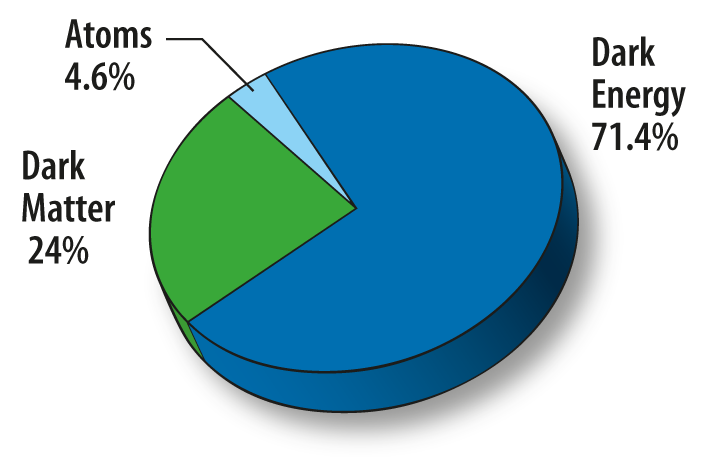
\includegraphics[width=0.7\textwidth]{Images/Background/universe_composition.png}
    \caption{To the best of our knowledge, the universe is composed of $5\%$ ordinary matter, $24\%$ dark matter, and $71\%$ dark energy. The Standard Model describes only ordinary matter, providing one indication that the model is not complete. Image altered from~\cite{universe_composition}.}
    \label{fig:universe_composition}
\end{figure}

Another problem is that gravity is not included in the Standard Model. Gravity is currently the least-understood fundamental force, and many questions about it remain to be answered, such as why gravity is so many orders of magnitude weaker than all the other forces. Attempts to unite the Standard Model with relativistic theories of gravity, as well as attempts to explain the relative weakness of gravity, has led to the development of fields such as string theory.

There is also the Higgs hierarchy problem, which relates to why the Higgs boson has the mass that it does~\cite{SUSY_primer}. To explain, let's say a particle has a certain "bare" mass. As it propagates through space, it interacts with other fields and particles in its environment, causing it to appear to have a different effective mass. Furthermore, in quantum interactions, particles are allowed to interact via "loops". In Figure~\ref{fig:quantum_loops} we see two particles interacting and then propagating away. In this case it is an acceptable interaction for one of the particles to loop around, so that its endpoint is the same as its start point. This particle is then known as a virtual particle, and the interaction is known as a loop interaction. To put it all together, as a particle propagates through empty space, it interacts with virtual particles via loop interactions, changing its observed mass. This observed mass is equal to the particle's bare mass plus contributions to its mass via loop corrections. If we calculate the expected mass of the Higgs, using what we know about how it interacts with other particles, we find that quantum loop corrections from virtual particles ought to be extremely large, with values around the Planck mass at $m_{Planck} = 10^{18}$ GeV. Some of these corrections are positive (for interactions with bosons) and some are negative (for interactions with fermions). For the Higgs to have an observed mass of 126 GeV, the bare mass and all of its corrections have to cancel each other out with an unnatural precision. This indicates that there is some additional undiscovered mechanism which is constraining the magnitude of the mass corrections.

\begin{figure}[htbp]
    \centering
    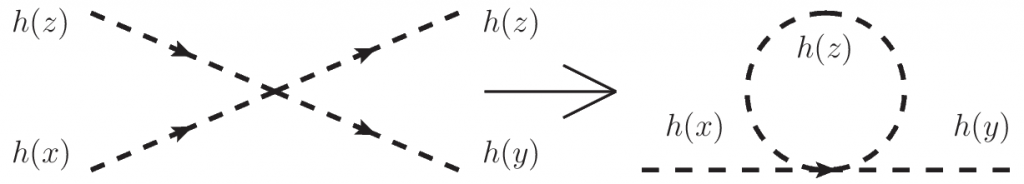
\includegraphics[width=0.9\textwidth]{Images/Background/loop_correction.png}
    \caption{On the left we see two particles interacting, where the x-axis is time. When one of the particles has the same start and end point, as seen on the right, the particle is known as a virtual particle and the interaction is known as a loop interaction. Interactions with virtual particles cause particles to get loop corrections to their observed mass. Image from~\cite{loop_correction}.}
    \label{fig:quantum_loops}
\end{figure}

All of these problems indicate that the Standard Model is not the culmination of physics. There are still things outside the Standard Model which have not yet been discovered. In particular, a class of extensions called supersymmetric (SUSY) theories have been proposed to solve many of the issues described in this section. We will now take a brief look at SUSY in order to understand what the theory proposes and why they are able to shore up various shortcomings of the Standard Model.